\section{Motivation für die Nutzung von RBF}
Es ist eine Lösung für das folgende Interpolationsproblem gesucht:\\
Es ist eine Menge von Trainingsdaten gegeben durch
\begin{equation*}
    M = \{(x^\mu,T^\mu) \quad | \quad x^\mu \in \mathbb{R}^m, T^\mu \in \mathbb{R}^n,\mu=1,\dots,p\}
\end{equation*}

\noindent Gesucht ist eine Funktion $g$, so dass gilt
\begin{equation*}
    %Was ist die undefined control sequence?!
    g: \mathbb{R}^m \to \mathbb{R}^n \quad \text{mit }g(x^\mu) = T^\mu \quad \forall \mu=1,\dots,p
\end{equation*}
\noindent Die Idee ist nun $g$ durch eine Linearkombination von p Funktionen $h_\nu(x) = h(\norm{x^\nu - x})$ mit belieb oft diff'barer radial symm. Funktion $h: \mathbb{R}^+ \to \mathbb{R}^+$\\
Das Interpolation wird also für $n=1$ bspw. durch
\begin{equation*}
    g(x^\mu)=\sum_{\nu=1}^p w_\nu h(\norm{x^\nu-x^\mu})=T^\mu \quad \forall \mu=1,\dots,p
\end{equation*}
gelöst. Die $w_\nu$ können analytischt bestimmt werden (siehe Skript Folie 125).

\subsection{Beispiele für radialsymm. Basisfunktionen}
Einige Beispiele für radialsymmetrische Basisfunktionen ($r=\norm{x-x^\mu})$
\begin{itemize}
    \item Gauss Funktion: $h(r) = \exp{(-\frac{r^2}{2\sigma^2})}$
    \item Inverse multiquadratische Funktion: $h(r) = \frac{1}{(r^2+c^2)^\alpha}$ mit $c\neq 0$ und $\alpha>0$
    \item Multiquadratische Funktion: $h(r) = (r^2+c^2)^\beta$ mit $c\neq0$ und $0<\beta\leq1$
\end{itemize}

\section{Aufbau eines RBF-Netzwerkes}
Im folgenden wird ein RBF Netzwerk beschrieben mit
\begin{itemize}
    \item $m$ Eingabeknoten
    \item $h$ RBF-Neuronen
    \item $n$ lineare Neuronen
\end{itemize}
Der Aufbau des Netzes ist in Abbildung \ref{ch_RBF_netz} zu sehen.

\begin{figure}[h]
    \centering
    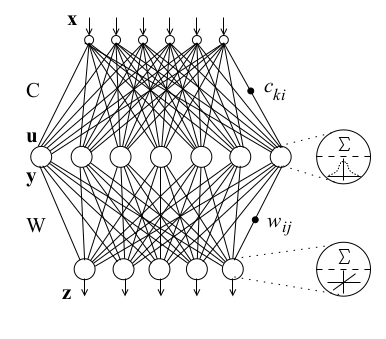
\includegraphics[width=0.4\textwidth]{img/RBF/RBFAufbau.png}
    \caption{RBF-Netzwerk}
    \label{ch_RBF_netz}
\end{figure}

Die Netzausgabe $z$ kann folgendermaßen berechent werden
\begin{align*}
    u_i &= \sqrt{\sum_{k=1}^m(x_k-c_{ki})^2} = \norm{x-c_i}\\
    y_i &= h(u_i)\\
    z_j &= \sum_{i=1}^h w_{ij}y_i [+\text{bias}_j]
\end{align*}

\section{Lernregel für RBF-Netzwerke}
Es wird nun eine Gradientenabstiegsverfahren für RBF-Netze hergeleitet
\begin{align*}
    \frac{\partial E}{\partial w_{ij}} &= \frac{\partial}{\partial w_{ij}}\norm{T-z}_2^2\\
    &= \frac{\partial}{\partial w_{ij}} \sum_j(T_j-z_j)^2\\
    &= -2(T_j-z_j)\frac{\partial}{\partial w_{ij}}\sum_i y_iw_{ij}\\
    &= -2y_i\delta_i
\end{align*}
Damit ergeben sich die folgenden Lernregeln\\
\paragraph{Online Modus}
\begin{align*}
    w_{ij}^{neu} &= w_{ij} - \eta_1 \frac{\partial E}{\partial w_{ij}} = w_{ij} + \eta_1 y_i\delta_j\\
    \text{bias}_j^{neu} &= \text{bias}_j - \eta_1 \frac{\partial E}{\partial w_{ij}}=\text{bias}_j +\eta_1\delta_j
\end{align*}

\paragraph{Batch Modus}

\begin{align*}
    w_{ij}^{neu} &= w_{ij} - \eta_1 \frac{\partial E}{\partial w_{ij}} = w_{ij} + \eta_1 \sum_\mu y_i^\mu\delta_j^\mu\\
    \text{bias}_j^{neu} &= \text{bias}_j - \eta_1 \frac{\partial E}{\partial w_{ij}}=\text{bias}_j +\eta_1\sum_\mu\delta_j^\mu
\end{align*}
Für die Gewichte der Eingabeschicht ergibt sich dann nach dem Backpropagation Algorithmus (siehe Skript für ausführliche Herleitung (Folie 130))

\begin{align*}
    \frac{\partial E}{\partial c_{ki}} &= \frac{\partial E}{\partial y_i}\frac{\partial y_i}{\partial c_{ki}}\\
    &= 2\sum_j\delta_jw_{ij}h'(u_i)\frac{1}{u_i}(x_k-c_{ki})
\end{align*}

Für gegebene RBF können dann konkrete Formen der Lernregel hergeleitet werden (siehe Skript Folie 131 ff.).

\subsection{Zusammenfassung: Lernalgorithmus (online) für RBF-Netze}
Es wird eine $m$-$h$-$m$ RBF-Netz behandelt. Als RBF wird $y=h(u) = \exp{(-\frac{u^2}{2\sigma^2})} = \exp{(-u^2s)}$. Es ist eine Menge von p gelabelten Mustern $(x^\mu,T^\mu)\in\mathbb{R}^m \times \mathbb{R}^n$ gegeben.\\

\paragraph{(1) Initialisierung}
Sinnvolle intialisierung der Gewichte $w_{ij}$ und $c_{ki}$.

\paragraph{(2) Berechnung der Netzausgabe z}
Für gegebenes Musterpaar $(x,T)$\\
\begin{align*}
    u_i^2 &= \sum_{k=1}^m(x_k-c_{ki})^2 \quad \text{für } i=1,\dots,h\\
    y_i &= \exp{(-\frac{u_i^2}{2\sigma^2})} \quad \text{für } i=1,\dots,h\\
    z_j &= \sum_{i=1}^hy_iw_{ij} \quad \text{für } j=1,\dots,n
\end{align*}

\paragraph{(3) Bestimme Fehler am Ausgang}
Berechne $\delta_j = (T_j - z_j)$ für $j=1,\dots,n$

\paragraph{(4) Lernen}
Adaptiere nach dem oben beschriebenen Lernregeln
\begin{align*}
    w_{ij}^{neu} &= w_{ij} +\eta_1y_i\delta_j\\
    c_{ki}^{neu} &= c_{ki} + \eta_2(x_k-c_{ki})y_is\sum_{j=1}^n\delta_jw_{ij}
\end{align*}
für $k=1,\dots,m$, $i=1,\dots,h$ und $j=1,\dots,n$

\paragraph{(5) Ende}
Gehe zurück zu Schritt (2), solange das Gütekriterium noch nicht erreicht wurde.

\section{Bemerkungen zu RBF-Netzen}
\begin{itemize}
    \item Anzahl der RBF-Neuronen ist kleiner als Anzahl der Trainingsmuster
    \item Vektor $c_i$ wird auch als Prototyp bzw. Zentrum bezeichnet
    \item Initialisierung der Gewichte $c_{ki}$ bspw. durch
        \begin{itemize}
            \item äquidistante Verteilung in Intervall $[\text{min},\text{max}]^m$
            \item durch Clusteranalyse
        \end{itemize}
    \item Verhalten des RBF-Netz hängt stark von der Wahl des Parameters $\sigma$ ab
    \item Parameter $\sigma_i$ kann für jedes RBF-Neuron $i$ individuell gewählt und auch adaptiert werden
    \item Adaption der Gewichte und $\sigma_i$ ist simultan oder sequentiell möglich
\end{itemize}

\subsection{Unterschiede MLP und RBF}
\begin{itemize}
    \item Klassifikation
        \begin{itemize}
            \item MLP: Trennen durch Hyperebenen
            \item RBF: Hyperkugeln umfassen Punkte der Klasse
        \end{itemize}
    \item bei MLP ist Repräsentation in verdeckter Schicht verteilt, bei RBF lokal
    \item Initialisierung der Gewichte bei MLP zufällig, bei RBF datenabhängig
    \item MLP und RBF können Funktionen beliebig genau approximieren
    \item schnellere Kovergenz mit RBF bei guter Initialisierung
\end{itemize}

\begin{figure}[h]
    \centering
    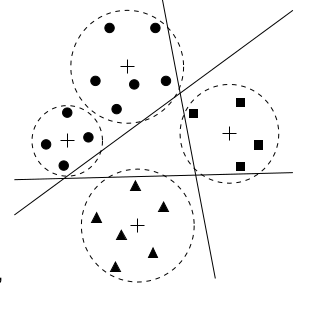
\includegraphics[width=0.4\textwidth]{img/RBF/MLPvsRBF.png}
    \caption{Klassifikation: MLP mit Hyperebenen vs. RBF mit Hyperkugeln}
    \label{ch_RBF_MLPvsRBF}
\end{figure}
